\section{Dipendenza della frequenza dalla lunghezza}
\label{sec:4}

Per studiare la proporzionalità inversa tra la frequenza di risonanza di secondo ordine e la lunghezza del tratto vibrante della corda, sono state effettuate misure mantenendo costante la tensione, data da una massa pari a $m = \qty{280.4 \pm 0.5}{\gram}$, e variando la lunghezza del tratto vibrante della corda. Le incertezze sono state stimate analogamente alle sezioni precedenti.
I dati raccolti sono riportati nella Tabella 3.

\begin{table}[H]
\centering
\begin{tabular}{ccc}
\hline
\textbf{Tratto vibrante} \textbf{(\unit{\meter})} & \textbf{Frequenza} \textbf{(\unit{\hertz})} & \textbf{Incertezza} \textbf{(\unit{\hertz})} \\
\hline
0.657 & 57.0 & 0.5 \\
0.822 & 46.0 & 0.5 \\
0.542 & 69.0 & 0.5 \\
0.411 & 92.0 & 0.5 \\
0.966 & 39.0 & 0.5 \\
1.123 & 33.0 & 0.5 \\
\hline
\end{tabular}
\caption{Frequenze misurate al variare della lunghezza del tratto vibrante della corda.}
\end{table}

Si procede interpolando linearmente le frequenze in funzione dell'inverso della lunghezza del tratto vibrante, come mostrato in Figura 3.

\begin{figure}[H]
    \centering
    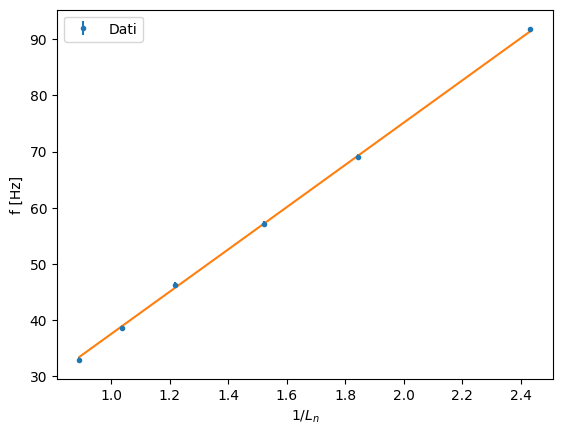
\includegraphics[width=0.6\textwidth]{Immagini/3.png}
    \caption{Interpolazione mediante minimi quadrati passante per l'origine: frequenza in funzione dell'inverso della lunghezza del tratto vibrante della corda.}
\end{figure}

Il test del $\chi^2$ mostra un buon accordo del modello lineare con i dati sperimentali, restituendo un $\Tilde{\chi}_o^2=0.61$, che per cinque gradi di libertà corrisponde ad una probabilità di accordo del 69.4\%.
Dalla relazione \eqref{eq:frequenze}, posto numero armonico n=2, segue che il coefficiente angolare interpolato è la velocità di propagazione delle onde sulla corda.\\ I valori ottenuti sono $v_2 = \qty{37.61 \pm 0.13}{\meter\per\second}$, mentre quello ricavato dalla relazione \eqref{eq:v-propagazione} è $v'_2 = \qty{36.2 \pm 1.7}{\meter\per\second}$. I due valori risultano compatibili, infatti tramite la relazione \eqref{eq:t_test} si è ottenuto $t_0 = 0.81$, che corrisponde a una probabilità di accordo del 41.8\%.

Si può inoltre confrontare questo valore di velocità con quello ottenuto nella sezione precedente, che è $v_1 = \qty{22.7 \pm 0.5}{\meter\per\second}$. La differenza tra i due valori è dovuta al fatto che in questa fase è stata utilizzata una massa maggiore per mantenere costante la tensione, pertanto la velocità di propagazione delle onde sulla corda risulta maggiore.